%----------------------------------------------------------------------------------------
% PACKAGES AND OTHER DOCUMENT CONFIGURATIONS
%----------------------------------------------------------------------------------------

\documentclass{beamer}

\usepackage{polski}
\usepackage[polish]{babel}
\usepackage[utf8]{inputenc}
\usepackage{lmodern}
\usepackage{graphicx}

\setbeamertemplate{frametitle}[default][center]

\begin{document}
  \begin{frame}
      \frametitle{Model komunikacji systemów w projekcie:}
      \center{,,Budowa rozproszonego systemu modelowania i sterowania instalacją
      CO na przykładzie dystrybucji ciepła w budynkach AGH''}
  \end{frame}
  
  \begin{frame}
    \frametitle{Architektura fizyczna}
    \center{Model komunikacji został oparty o architekturę scentralizowaną, w
    której obecni w systemie klienci komunikują się wyłącznie za pośrednictwem
    wspólnego serwera}
    
    \begin{figure}[!htb]
      \begin{center}
        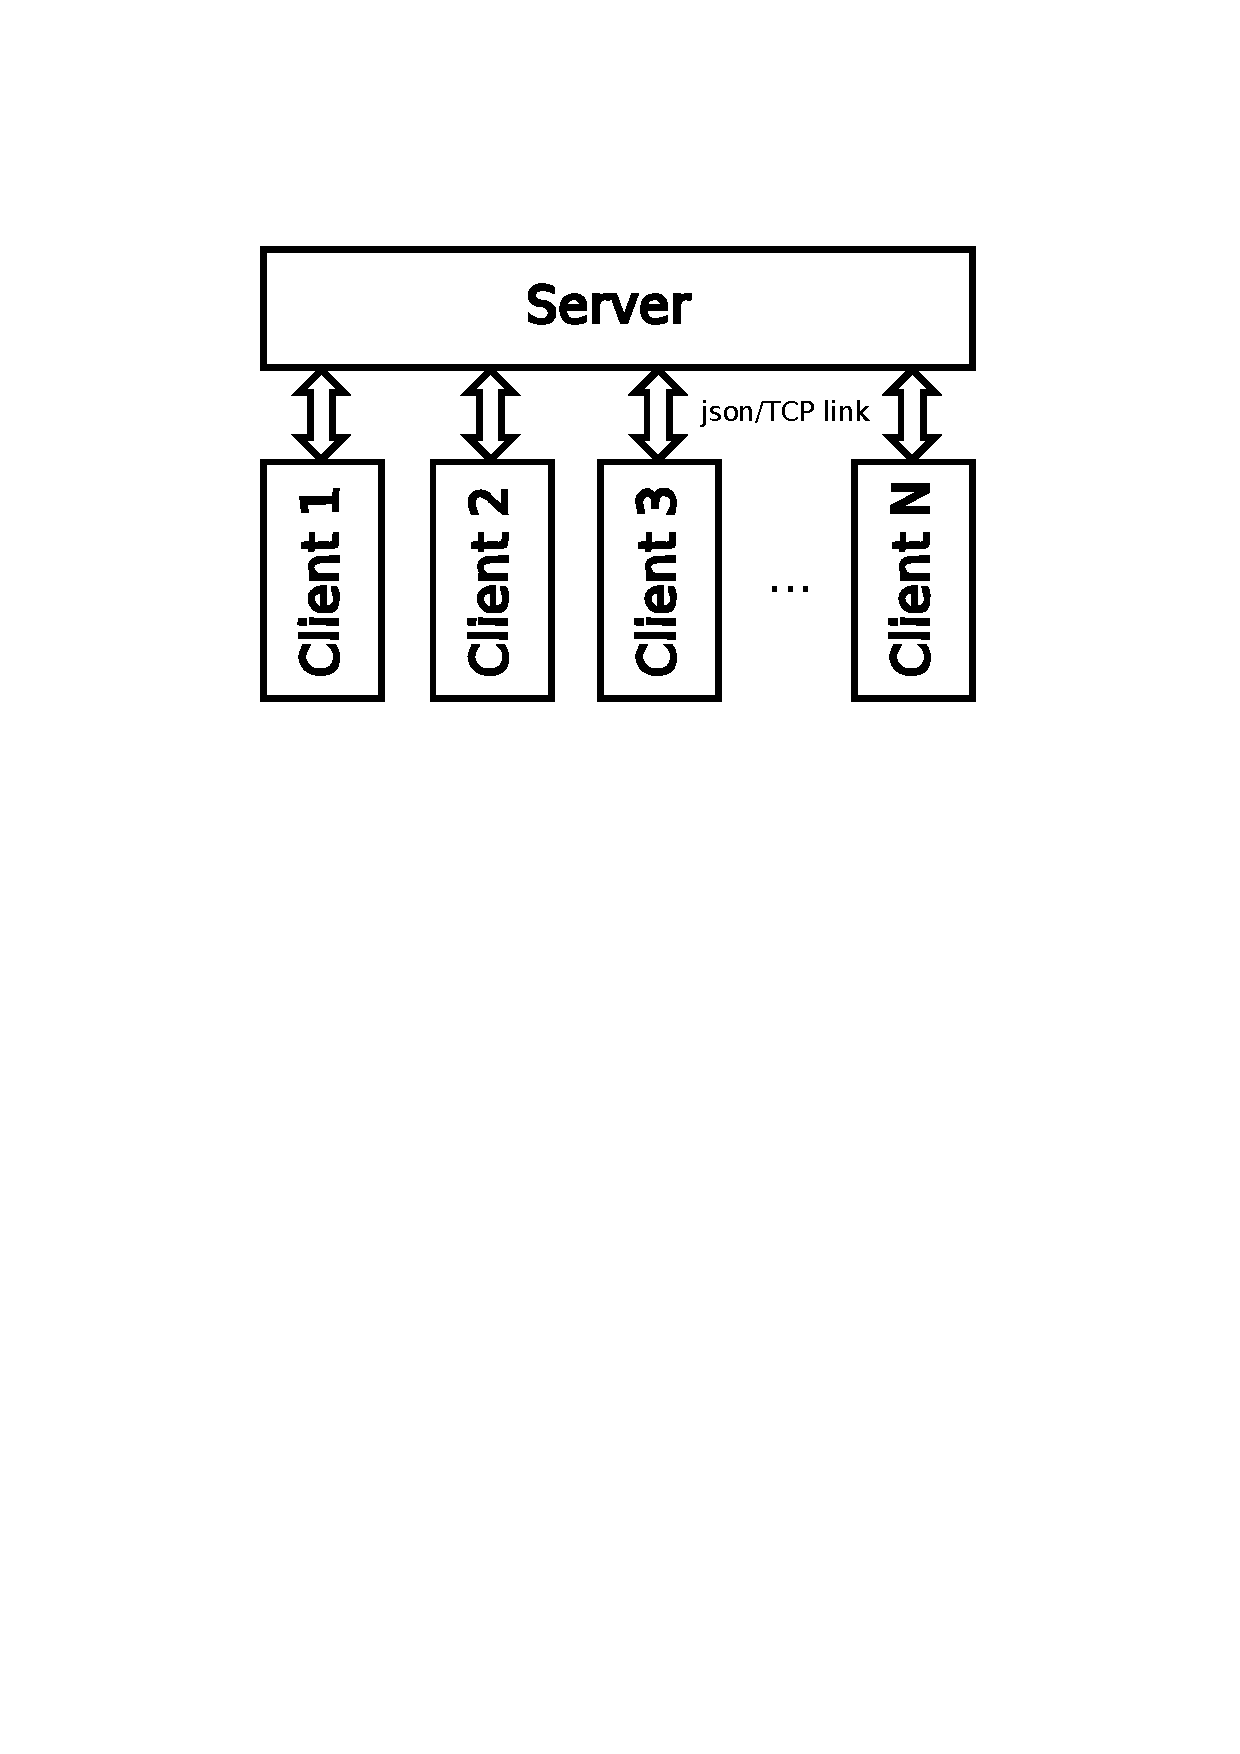
\includegraphics[width=6cm,trim=4cm 17.5cm 4cm 4cm,clip]
        {../res/img/arch_diagram.pdf}
      \end{center}
      \caption{Architektura modelu komunikacji}
      \label{plot:x1}
    \end{figure}
  \end{frame}
  
  \begin{frame}
    \frametitle{Architektura fizyczna, wady i zalety}
    Wady:
    \begin{itemize}
      \item <1-> Awaria serwera oznacza awarię całego systemu(nawet jeśli
      wszyscy klienci działają poprawnie)
    \end{itemize}
    Zalety:
    \begin{itemize}
      \item <1-> Klient utrzymuje tylko jedno połączenie TCP
      \item <1-> Serwer jest naturalnym miejscem do logowania historii
      eksperymentu
      \item <1-> Rozbudowanie istniejącego systemu o dodatkowe funkcjonalności
      jest prostsze niż w przypadku systemu rozproszonego
    \end{itemize}
  \end{frame}
  
  \begin{frame}
    \frametitle{Architektura logiczna}
    Komunikacja serwera z klientami polega na wymianie obiektów w formacie
    \textit{JSON} poprzez protokół \textit{TCP}. Działanie systemu składa się z
    dwóch faz:
    \begin{enumerate}
      \item <1-> Inicjalizacja
      \item <1-> Symulacja
    \end{enumerate}
  \end{frame}
  
  \begin{frame}
    \frametitle{Architektura logiczna, Inicjalizacja}
    W tej fazie serwer oczekuje na połączanie wszystkich zadeklarowanych w pliku
    konfiguracyjnym klientów. Po spełnieniu tego warunku rozsyła do nich
    pakiet inicjalizacyjny, który kończy tę fazę, i powoduje przejście do fazy
    \textit{Symulacja}
  \end{frame}
  
  \begin{frame}
    \frametitle{Architektura logiczna, Symulacja}
    Na tę fazę składają się następujące operacje:
    \begin{enumerate}
      \item <1-> Zebranie wyników od klientów
      \item <1-> Rozesłanie przefiltrowanych wyników do klientów
      \item <1-> Diagnostyka serwera
      \item <1-> Powrót do kroku 1
    \end{enumerate}
    Faza ta działa w trybie iteracyjnym, każdy krok symulacji oznacza wykonanie
    pełnej iteracji w fazie symulacji. Podczas każdej iteracji w kroku 4
    serwer sprawdza, czy połączenia z klientami są utrzymane, w przeciwnym
    wypadku wraca do fazy \textit{Inicjalizacja}
  \end{frame}

\end{document}
